\documentclass[addpoints]{physlabs}  % Add the answers option to print answers to prelab and postlab exercises.

\labtitle{Understanding Statistical Uncertainties}
\labnum{1}
\labnumroman{I}
\course{PHYSICS 113 - 121 - 181}
\coursesubtitle{General Physics I and Mechanics}
\date{\today}

\begin{document}

\maketitle
% PRELAB SECTION
\begin{prelab}

\question[2] You are trying to see if there is a pattern to when spam arrives in your mailbox, so you count the number of spam emails over the last month and bin them according to which time of day they were sent.
Out of 1595 spam emails, 784 were received during the day, between 6 AM and 6 PM.
Treating spam emails as Poisson distributed, explain if your data support the idea that spammers prefer one part of the day over the other?
\textit{Hint: add error bars to the data and see if there is overlap.}
\begin{solution}[3cm]
\end{solution}

\question[2] You choose to investigate a bit more diligently and further subdivide the day into four equal time intervals.
What conclusion do you draw from your data now, and why?

\begin{center}
\begin{tabular}{c|c}
    Time of day & No.\ of spam emails \\ \hline
    midnight to 6:00 AM  & 383 \\
    6:01 AM to noon      & 401 \\
    noon to 6:00 PM      & 374 \\
    6:01 PM to midnight  & 447
\end{tabular}
\end{center}

\textcolor{red}{(this question is from the previous prelab. Still want to keep it? the form of this problem is a little bit strange, the table goes to the end)}
\begin{solution}[3cm]
\end{solution}

\question[2] You are a quality engineer for a paper company, and need to ensure that the area of A4 sheets being produced has less than $0.1\%$ area error.
 You analyze a sample of A4 paper and find the width and length statistics to be, respectively, $210\pm 0.2$mm and $297\pm 0.3$mm.
 Does the company have a problem, or not? Explain.
\begin{solution}[3cm]
\end{solution}

\end{prelab}

% LAB SECTION
\begin{labsection}

\begin{objective}
To understand common statistics used to describe data and their estimators.
To become familiar with the quick estimation of measurement uncertainties and their propagation into derived quantities.
\end{objective}

\begin{theory}
\subsection*{Introduction}
Throughout this semester you will perform experiments which involve measurements.
Any device you use is imperfect and won't give you infinitely precise results.
Your measurements will include the true value sought after muddied by the measurement errors due to these imperfections.
Understanding errors is crucial in being able to extract the true value from these imperfect measurements.
Sometimes errors are big, sometimes small - understanding errors means understanding how they are distributed.


You are probably familiar with elections and polling.
During an election, each voter has a preference; there is a \textit{distribution} of preferences across the population.
During the election we learn what that distribution is, and a \textit{statistic}, the winner, is determined.
Prior to an election, polls attempt to predict this statistic, they are \textit{estimators} of the statistic.
They do this by \textit{sampling} a fraction of the population.
If the sample is carefully chosen to represent the population, then the estimator is \textit{unbiased}.
This does not mean that the poll predicts the election results exactly, but that the error in the estimator's prediction depends on the sample size.
The larger the sample, the closer the prediction is to the actual election result, decreasing the \textit{statistical error}.
If the sample is not chosen properly, then the estimator is \textit{biased}.
The prediction will have a \textit{systematic error} that does not go away as the sample size is increased.

The difference between a good and a bad experiment depends on understanding systematic and statistical errors.
Distributions are useful tools in experiments that involve counting.
When counting \textit{discrete} stuff, like the number of lightning bolts every hour during a storm, then a \textit{probability distribution} tells you the chance you have of observing one, two, or even a hundred, strikes.
These are typically represented with a $p_n$ where $n$ runs over the discrete possibilities.
When counting \textit{continuous} quantities, like the amount of time between successive lightning strikes, then a \textit{probability density function} (pdf) tells you the chance you have of seeing a lightning bolt in any time interval, such as waiting up to eight minutes, or more than 10.5, or somewhere between the two!
These are typically represented as $\rho(x)$ where $x$ runs over the continuous values.




\subsubsection*{Common Statistics and their Unbiased Estimators}
The most common, and useful, statistic is the \textit{mean} (or \textit{average}).
Let $X$ be the collection of all possible outcomes in an experiment.
A particular outcome in the set of all possible outcomes is written $x\in X$.
The mean for discrete or continuous distributions is, respectively,
\begin{equation*}
    \mu = \sum_{x\in X}p_x x\hspace{10pt}\text{or}\hspace{10pt}\int_X \!\!\!dx\ \rho(x) x.
\end{equation*}
The spread in a distribution is captured by the second most important statistic, the \textit{variance},
\begin{equation*}
    \sigma^2 = \sum_{x\in X} p_x(x-\mu)^2\hspace{10pt}\text{or}\hspace{10pt}\int_X \!\!\!dx\ \rho(x) (x-\mu)^2,
\end{equation*}
the square root of which, $\sigma$, is the \textit{standard deviation}.
In other contexts you will see these statistics sometimes written using \textit{expectation} symbols, $\mu=\mathds{E}[X]$ and $\sigma^2=\mathds{E}[(X-\mathds{E}[X])^2]$, or other times with angle brackets, $\mu=\langle x\rangle$ and $\sigma^2=\langle(x-\langle x\rangle)^2\rangle$.
If there are multiple types of outcomes, say $X$ and $Y$, then subscripts are added to distinguish means, $\mu_X$ and $\mu_Y$, or variances, $\sigma_X^2$ and $\sigma_Y^2$.

If $X$ and $Y$ are dependent random variables, then our final important statistic is the \textit{covariance},
\begin{align*}
    \sigma_{XY}=\sum_{x\in X}\sum_{y\in Y}p_{x,y}(x-\mu_X)(y-\mu_Y)\hspace{10pt}\text{or}\hspace{10pt}\int_X \!\!\!dx\!\! \int_Y \!\!\!dy\ \rho(x,y) (x-\mu_X)(y-\mu_Y),
\end{align*}



In any case, the formulas presented above are great for theoretical purposes, but not for experimental ones.
The reason is probability distributions and pdf's, like true preference distributions prior to elections, are not known a priori, so you cannot actually compute these statistics most of the time.
Fortunately, a sample of $N$ measurements, $s=\{x_1,x_2,\dots,x_N\}$, can be used to estimate these statistics.
We call $X$ \textit{data}.
The unbiased estimator of the mean is
\begin{align}
    \hat\mu = \frac{1}{N}\sum_{n=1}^N
x_n\end{align}
and for the variance
\begin{align}
    \hat\sigma^2 = \frac{1}{N-1}\sum_{n=1}^N(x_n-\hat \mu)^2.
\end{align}
Notice the estimators have little hats (the technical name is circumflex) on them to distinguish them from the true statistics.
The estimator of the standard deviation is typically quoted as the error in estimator of the mean, written $\hat\mu\pm\hat\sigma$, $\hat\mu(\pm\hat\sigma)$, or $\hat\mu^{\pm\hat\sigma}$.
These two statistics are what you will compute from your data.
If you're not acquainted with how to use the formulas, then make sure you are by the time the lab starts.
You will be using them for years to come.

\subsection*{Error Propagation}
Say you measure $x$ and $y$, so your data consists of tuples $(x_i,y_i)$ for $i=1,2,\dots,N$.
You are actually interested in learning about another quantity $z$ that depends on $x$ and $y$ though some function $f$,
\begin{equation}
    z = f(x,y).
\end{equation}
Since the quantities are related, their statistics are also related.
Suppose you've estimated $\hat\mu_x\pm\hat\sigma_x$ and $\hat\mu_y\pm\hat\sigma_y$.
Can you use these to get $\hat\mu_z\pm\hat\sigma_z$?

If the estimated standard deviations of $x$ and $y$ are both small compared to their means, $\hat\sigma/\hat\mu<0.1$, and the function $f$ is reasonably well-behaved, then yes!
The mean of $z$ is estimated to be $\hat\mu_z=f(\hat\mu_x,\hat\mu_y)$.
The variance is
\begin{align}
    \hat{\sigma}_z^2 \approx \left(\frac{\partial f}{\partial x}\right)^2\hat\sigma_x^2+\left(\frac{\partial f}{\partial y}\right)^2\hat\sigma_y^2,
\end{align}
with the derivatives evaluated at the estimated means.

\subsection*{Special Distributions}
\begin{center}
\textit{Poisson Distribution}
\end{center}
The Poisson distribution is one of the most important discrete distributions, and is used when counting rare events.
If a random event occurs independently of when it last occurred, and events occur at a fixed average rate, then the random events are described by a Poisson distribution.
During a lightning storm it is acceptable to treat each lightning strike as an independent event.
During the full length of the storm a set number of strikes occured, so there is some average rate of occurrence, $\alpha$.
Divide up the length of the storm into time intervals $\Delta t$.
Then you expect to see $N=\alpha \Delta t$ strikes per interval, on average.
Since the strikes are random and independent, in some intervals you will see more than $N$, while in others you will see less.
The probability that you see $n$ strikes in an interval is
\begin{align}
    p_n=\frac{N^n}{n!}e^{-N}.
\end{align}
Since the mean and variance of this distribution are both equal to $N$, it is valid to say that you expect to see $N\pm\sqrt{N}$ lightning strikes in your $\Delta t$ time intervals.
This is a good rule of thumb to remember - the error in counting experiments can quickly be estimated by taking the square root of the mean.


\end{theory}
\begin{equipment}
    \item $1/2$ meter stick
    \item Geiger Counter \& Wand
\end{equipment}

\textcolor{red}{(Maybe add some pictures of Geiger counter, the 3 plates and how to set up properly)}

\begin{experiment}
\subsection*{Experiment 1: The Psychophysics of Reacting to Visual Stimuli}
In this experiment you and your partner will measure each other's reaction times without a stopwatch.
One of you will drop a ruler for the other to catch.
The location of the grasping hand is a measurement of how far the ruler dropped.
Since the ruler starts out at rest, the height it falls, $h$, in a time interval, $t$, is the kinematical formula
\begin{align}
    h = \frac{1}{2}g t^2 \hspace{10pt}\text{  where  }\hspace{10pt} g = \qty{9.81}{\frac{\meter}{\second^2}}
\end{align}
is the gravitational acceleration at the surface of the Earth.
So a measurement of $h$ can be transformed into a measurement of $t$.
\begin{enumerate}
    \item You and your partner choose the unique roles of either \textbf{Lab Partner A} or \textbf{Lab Partner B}.
    \item \textbf{Lab Partner A}: Hold the ruler vertically with the \qty{50}{\centi\meter} end at the top, as high up as possible.
    \item \textbf{Lab Partner B}: Position your open hand at the lower end of the ruler, not touching it.
    Line up the top of your hand with the \qty{0}{\centi\meter} mark, say ``Ready," and begin waiting.
    Keep your eyes on your hand.
    \item \textbf{Lab Partner A}: After hearing your partner say ``Ready," respond with ``Set," and wait however long you like.
    Without warning, let go of the ruler.
    \item \textbf{Lab Partner B}: As soon as you notice the ruler dropping, close your hand to catch it.
    Once caught, show your clenched hand to you partner.
    (Practice steps 3-5 until you both feel comfortable doing it).
    \item \textbf{Lab Partner A}: find the ruler mark that is just visible at the top of your clenched hand, and record the value of $h_1$ in the Post-lab.
    \item Repeat steps 2-6 24 more times, except now recording $h_2, h_3,\dots, h_{25}$.
    \item Switch the roles of \textbf{Lab Partner A} and \textbf{Lab Partner B}, and repeat steps 2-7.
    \item Perform experiment 2 before starting work on the post-lab questions.
\end{enumerate}

\subsection*{Experiment 2: Radioactive $\beta$-Decay}

\begin{center}
    
\includegraphics[width=0.5\linewidth]{Lab 01: Statistics and Error Propagation/Strontium_Decay.jpeg}
    \captionof{figure}{Cartoon showing the decay chain of \ce{^{90}Sr} to \ce{^{90}Y} and \ce{^{90}Zr}, producing two $\beta^-$ particles (electrons) and two anti-neutrinos:
    \begin{displaymath}
        \ce{^90_38Sr} \to \ce{^90_39Y} + e^- + \bar{\nu}_e, \qquad \text{28.8-year half-life},
    \end{displaymath}
    \begin{displaymath}
        \ce{^90_39Y}  \to \ce{^90_40Zr} + e^- + \bar{\nu}_e, \qquad \text{64-hour half-life}.
    \end{displaymath}
    Inside the nucleus, a neutron decays to a proton during each beta decay, increasing the atomic number from $38\to39\to40$ and very slightly decreasing the atomic mass.\label{fig: sr decay chain}}
\end{center}

In this experiment, you will count the number of $\beta$-particles (electrons) emitted by a source of radioactively decaying \ce{^{90}Sr} (strontium-90). \ce{^{90}Sr} atoms have a half-life of 28.8 years and decay into \ce{^{90}Y} (yttrium-90) by emitting an electron ($\beta^-$) and an antineutrino ($\overline{\nu}_e$) in a process called $\beta$-\textsl{decay} (see Fig.~\ref{fig: sr decay chain}). \ce{^{90}Y} atoms have a half-life of 64 hours and decay into stable \ce{^{90}Zr}, emitting another $\beta^-$ and $\overline{\nu}_e$.
It is these $\beta$-rays that you will be counting.

The \ce{^{90}Sr} sample is a small button sealed within a protective steel frame. The frame blocks the vast majority of emitted electrons, so your net radiation exposure will be less than when you take a flight across the United States. A Geiger counter with an external wand is used to measure the radiation coming off the sample. Since the sample emits $\beta$ particles at a fixed rate and independently of when the last particle was emitted, this can be treated as a Poisson process. You will measure how many particles are emitted per second using three different setups, and then look at how the statistical uncertainty in the number of counts varies with the number of trials.

\begin{enumerate}
\item Turn the Geiger counter on. The counter will make a rapid clicking sound when placed near the sample; you may turn off the volume of the counter if you wish.
Set it to take $1$ second readings, and test it by placing the wand very near the source with no objects between the two.
If you are not reading at least $100$ counts per second, talk to your TA.
\item Examine the steel box containing the sample, and play around with inserting the different plates and the wand.
In the postlab sketch the inside of the steel box, showing how the wand and plates appear when fully inserted.
Don't forget to label parts.
\item With nothing between the wand and the source, take $10$ readings and log your measurements in the post-lab.
\item Place the \qty{0.12}{\milli\meter} aluminum plate between the wand and the source, take $10$ readings and log your measurements in the post-lab.
\item Remove the thin plate and place the thicker \qty{0.60}{\milli\meter} aluminum plate between the wand and the source, take $10$ readings and log your measurements in the post-lab.
\item Go back to your sketch of the inside of the box and add where you think the radioactive source is. Label the added source.
\item Work on the post-lab questions.


\end{enumerate}
\end{experiment}

\end{labsection}

\begin{postlab}

\begingradingrange{exp1}
\fullwidth{\subsection*{Experiment 1 (12 points)}}

\question[3] For each $h_i$ recorded during the experiment, calculate the corresponding $t_i$ value in the table below in milliseconds. Pay attention to units.

\textcolor{red}{(Draw vertical lines for each column)}

\begin{center}
    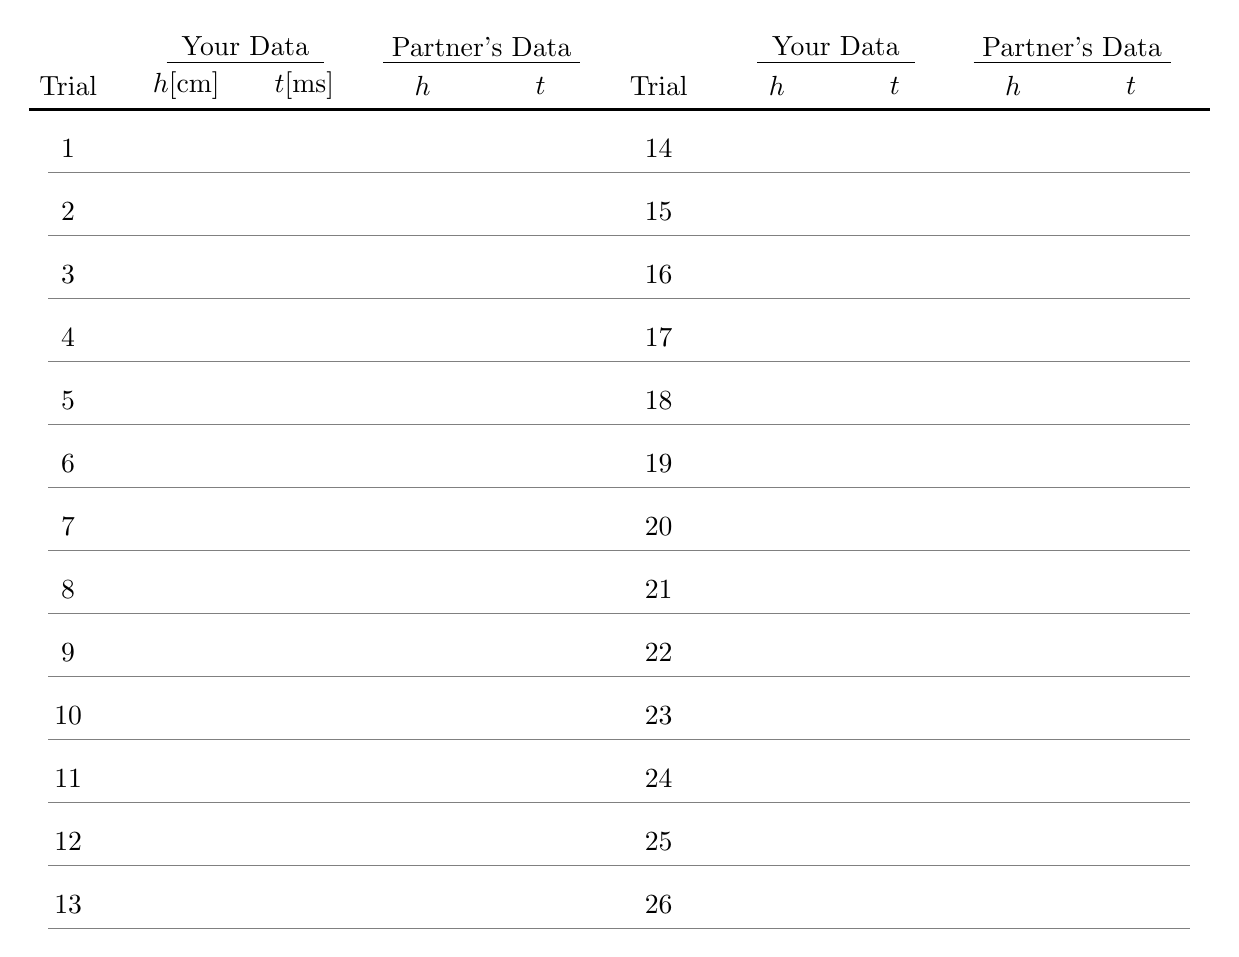
\begin{tikzpicture}
        \begin{scope}[]
        % Table headers
        \node at (0, 0.3) [] {Trial};
        \node at (2.25, 0.8) [] {Your Data};
        \node at (1.5, 0.3) [] {$h$[cm]};
        \node at (3, 0.3) [] {$t$[ms]};
        \node at (5.25, 0.8) [] {Partner's Data};
        \node at (4.5, 0.3) [] {$h$};
        \node at (6, 0.3) [] {$t$};
        \node at (7.5, 0.3) [] {Trial};
        \node at (9.75, 0.8) [] {Your Data};
        \node at (9.0, 0.3) [] {$h$};
        \node at (10.5, 0.3) [] {$t$};
        \node at (12.75, 0.8) [] {Partner's Data};
        \node at (12, 0.3) [] {$h$};
        \node at (13.5, 0.3) [] {$t$};
        % Draw horizontal line under headers
        \draw[thick] (-0.5, 0) -- (14.5, 0);
        \draw (1.25, 0.6) -- (3.25, 0.6);
        \draw (4.00, 0.6) -- (6.5, 0.6);
        \draw (8.75, 0.6) -- (10.75, 0.6);
        \draw (11.50, 0.6) -- (14.0, 0.6);

         % Empty rows for data entry
        \foreach \row in {1,...,13}
        {
            \node at (0, 0.3-0.8*\row) {\row};
            \pgfmathsetmacro{\trialnum}{int(\row+13)}
            \node at (7.5, 0.3-0.8*\row) {\trialnum};
            \draw[color=gray] (-0.25, -0.8*\row) -- (14.25, -0.8*\row);
        }
        \end{scope}
    \end{tikzpicture}
\newpage
    \vspace{20pt}
    
\begin{tikzpicture}
        % Define dimensions
        \def\gridwidth{32}
        \def\gridheight{15}
        \def\spacing{0.5}
        % Draw grid paper on the left
        \begin{scope}[xshift=0cm,yshift=0cm]
            % Major grid lines (thicker)
            \foreach \x in {0,1,...,\gridwidth}
                \draw[gray,thick] (\x*\spacing,0) -- (\x*\spacing,\gridheight*\spacing);
            \foreach \y in {0,1,...,\gridheight}
                \draw[gray, thick] (0,\y*\spacing) -- (\gridwidth*\spacing,\y*\spacing);
            \draw[black, very thick] (0,0) rectangle (\gridwidth*\spacing,\gridheight*\spacing);
        \end{scope}
    \end{tikzpicture}
\end{center}

\question[3] Use the graph above to draw two cumulative distribution functions for you and your partner's reaction times. You will have to determine what bin size to use based on your data.
Don't forget to add axes, labels, units, and a title.
In future plots you will not be reminded.

\question[3] Calculate the means and standard deviations of the two data samples you collected.
Make sure you don't forget units.
Write them in the form $\mu\pm\sigma$:
\begin{table}[h]
    \centering
    \begin{tabular}{c|c|c}
         & Your Values & Partner's Values\\
         \hline & & \\
         Height &  $\pm$ &  $\pm$\\ & & \\
         \hline & & \\
         Time &  $\pm$ &  $\pm$\\ & & \\
    \end{tabular}
    \label{tab:placeholder}
\end{table}

\question[3] Use error propagation to compute the variance in your $t$ measurements. How does it compare to the error you computed in the previous question?

\endgradingrange{exp1}
\fullwidth{\subsection*{Experiment 2 (12 points)}}
\begingradingrange{exp2}

\question[2] Record your Geiger counter readings in the table below and sketch the inside of the steel box.

\begin{center}
    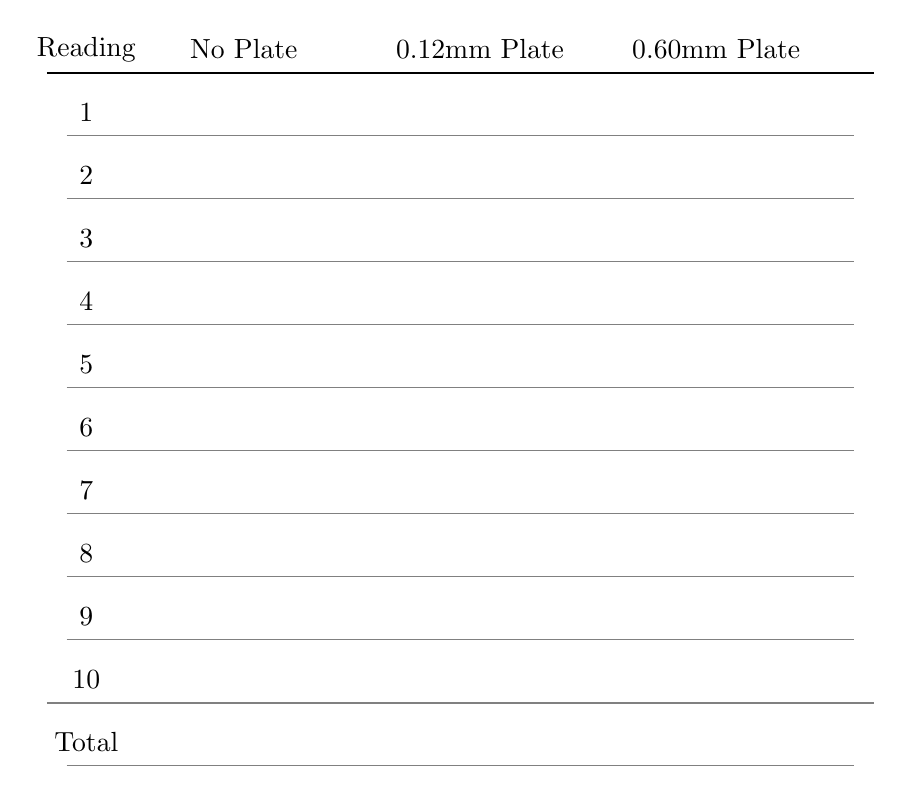
\begin{tikzpicture}
    \begin{scope}[]
    % Table headers
    \node at (0, 0.3) [] {Reading};
    \node at (2, 0.3) [] {No Plate};
    \node at (5, 0.3) [] {$0.12$mm Plate};
    \node at (8, 0.3) [] {$0.60$mm Plate};
    % Draw horizontal line under headers
    \draw[thick] (-0.5, 0) -- (10, 0);
     % Empty rows for data entry
    \foreach \row in {1,...,10}
    {
        \node at (0, 0.3-0.8*\row) {\row};
        \draw[color=gray] (-0.25, -0.8*\row) -- (9.75, -0.8*\row);
    }
    \draw[thick,color=gray] (-0.5, -0.8*10) -- (10, -0.8*10);
    \node at (0, 0.3-0.8*11) {Total};
        \draw[color=gray] (-0.25, -0.8*11) -- (9.75, -0.8*11);
    \end{scope}
\end{tikzpicture}
\end{center}

\textcolor{red}{(Draw vertical lines for each column)}

Sketch of the steel box inside:
\vfill
\textcolor{red}{(the space to draw may be small)}
\newpage

\question[2] Consider your data for just the first reading in each of the three setups. What is the statistical error in each? Does your first reading distinguish between the three setups? Explain why.

\question[2] Now add up all the readings and fill in the last line of your data chart. What is the error now for each of the three setups? Does your combined data distinguish between the three setups? Explain.

\question[2] For each setup count the number of readings that fall within one error bar. Within 2 error bars? Make a chart.

\question[3] Compare the errors between the first reading and the total data. Is the ratio of these two errors what you expect?
Explain.
What do you expect the errors to be for $100$ readings instead of $10$? $1000$ readings?

\question[1] If you design an experiment to unambiguously discern between the no plate and $0.12$mm plate setups, how many readings do you require? Explain.

\endgradingrange{exp2}

\end{postlab}

\end{document}
